\subsubsection{Satisfaction Measures}\label{sec:satisfactionmeasures}
We measure the groups' satisfaction of a recommended list, $\omega$, according to Normalized Discounted Cumulative Gain(nDCG). We used two different variations which are described in this section. nDCG is used for measuring the quality of ranked lists against user preferences, which is commonly used within the information retrieval field for comparing ranked lists of queries\cite{ndcg}.

%\subsubsection{Satisfaction Measures}
\adparagraph{nDCG}
Figure \ref{fig:ndcg} shows the nDCG score for BC, MC, SF, and Avg. With nDCG a higher score is better as covered in Section \ref{sec:methodology_ndcg}.
BC and MC gets the best results, but they all follow the same general trend with a sharp decrease in score that quickly levels out.

One outlying case SF starts out close to Avg for a group size of four, but decreases much less in score and is closer to BC and MC as the size increases.

\begin{figure}[H]
	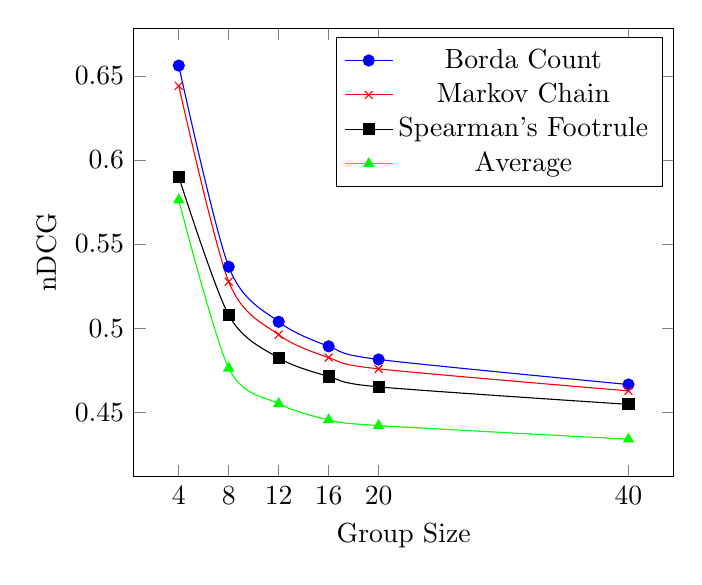
\begin{tikzpicture}
	\begin{axis}[
	xlabel=Group Size,
	ylabel=nDCG,
	xtick = {4,8,12,16,20,40}]
	\addplot[smooth,mark=*,blue] plot coordinates {
		(4,0.6561)
		(8,0.5365)
		(12,0.5038)
		(16,0.4892)
		(20,0.4814)
		(40,0.4665)
	};
	\addlegendentry{Borda Count}
	
	\addplot[smooth,color=red,mark=x] plot coordinates {
		(4,0.6440)
		(8,0.5276)
		(12,0.4961)
		(16,0.4825)
		(20,0.4758)
		(40,0.4627)
	};
	\addlegendentry{Markov Chain}
	
	\addplot[smooth,color=black,mark=square*] plot coordinates {
		(4,0.59)
		(8,0.5077)
		(12,0.4823)
		(16,0.4713)
		(20,0.4651)
		(40,0.4547)
	};
	\addlegendentry{Spearman's Footrule}
	
	\addplot[smooth,color=green,mark=triangle*] plot coordinates {
		(4,0.5762)
		(8,0.4762)
		(12,0.4551)
		(16,0.4455)
		(20,0.4421)
		(40,0.434)
	};
	\addlegendentry{Average}
	
	\end{axis}
	\end{tikzpicture}
	\caption{Results for nDCG test}\label{fig:ndcg}
\end{figure}
\subsubsection{Distance Measures}

\paragraph{Kendall Tau Distance}
\note{This is a rough draft}
Kendall tau distance is a measure of the difference between ranked lists\citep{rank:aggregation}. It counts the pairwise disagreement between two ranked lists as specified in the Equations \ref{eq:kendalldistance1}, \ref{eq:kendalldistance2} and \ref{eq:kendalldistancefinal}. The count is then normalized by dividing with $n(n-1)/2$ where $n$ is the total number of available positions, giving the maximum number of possible values. \note{check up on this}
These two equations are used when working with full lists where every list contains every item. 

\begin{equation}\label{eq:kendalldistance1}
K1(\sigma,\tau) = | \{(i,j) | i < j, \sigma (i) < \sigma (j) \land \tau (i) > \tau (j)|
\end{equation}
\begin{equation}\label{eq:kendalldistance2}
K2(\sigma,\tau) = | \{(i,j) | i < j, \sigma (i) > \sigma (j) \land \tau (i) < \tau (j) \} |
\end{equation}

\begin{equation}\label{eq:kendalldistancefinal}
K(\sigma,\tau) = k2(\sigma,\tau) + k1(\sigma,\tau)
\end{equation}

The above measure is for full lists but as we work on top-k lists we have found a modification of the standard Kendall tau distance\cite{comparing:topk}. 

 which we do by adding a third case in which it needs to count a disagreement. If a item occurs on one list but not the other it is assigned the value of the total number of items plus 1. We then add Equation \ref{eq:kendalldistance3} to Kendall tau distance in case we encounter equal items on one list which is undesirable.

\begin{equation}\label{eq:kendalldistance3}
K(\sigma,\tau) = | \{(i,j) | i < j, \sigma (i) = \sigma (j) \lor \tau (i) = \tau (j) \} |
\end{equation}

To find the distance from a recommended list to a groups preferences each list of user preferences are compared to the result list and the average distance is the result. 



\paragraph{Spearman Distance}